\documentclass{article}

\usepackage{xcolor}
\usepackage{comment}
\usepackage{graphicx}
\usepackage{csquotes}
\usepackage{balance}
\usepackage{setspace}

\usepackage{listings}
\usepackage{subcaption}

\usepackage{standalone}
\lstset{ %
language=C++,                % choose the language of the code
basicstyle=\ttfamily\footnotesize,       % the size of the fonts that are used for the code
columns=fullflexible,
numbers=left,                   % where to put the line-numbers
numberstyle=\footnotesize,      % the size of the fonts that are used for the line-numbers
stepnumber=1,                   % the step between two line-numbers. If it is 1 each line will be numbered
numbersep=5pt,                  % how far the line-numbers are from the code
%backgroundcolor=\color{codeBG3},  % choose the background color. You must add \usepackage{color}
showspaces=false,               % show spaces adding particular underscores
showstringspaces=false,         % underline spaces within strings
showtabs=false,                 % show tabs within strings adding particular underscores
frame=single,           % adds a frame around the code
tabsize=2,          % sets default tabsize to 2 spaces
captionpos=b,           % sets the caption-position to bottom
breaklines=true,        % sets automatic line breaking
breakatwhitespace=false,    % sets if automatic breaks should only happen at whitespace
keywordstyle=\color{blue},       % keyword style
  %language=Octave,                 % the language of the code
  otherkeywords={SearchVar,MV,TSS,tileExpr,Search,tFunc...},           % if you want to add more keywords to the set
  numberstyle=\tiny\color{black}, % the style that is used for the line-numbers
  rulecolor=\color{black},
escapeinside={<@}{@>}
}

\newcommand{\todo}[1]{{\textcolor{red}{{\tt{TODO:}}\,\,#1 }}}
\newcommand{\nc}[0]{\todo{cite}}
\newcommand{\an}[1]{{\textcolor{blue}{Author's Note: #1}}}
\newcommand{\ttt}[1]{{\texttt{#1}}}

\author{Brandon Neth}
\title{Dissertation Proposal}

\begin{document}
\maketitle

\begin{abstract}
    good stuff.
\end{abstract}



\section{Introduction}
From optimizing wind-farm performance~\cite{sprague2020exawind} to understanding the dynamics of the watershed~\cite{olschanowsky2019hydroframe}\todo{cite parflow},
high-performance computing (HPC) is a critical strategy for combatting the climate crisis. 




When developing such applications, domain scientists often encounter the need to optimize or otherwise refactor their application code. 
Generally, they have two options: learn how to optimize their code themselves or enlist the help of software engineers. 
\todo{write off the enlisting a programmer line in a short sentence.} 
For those that choose to tackle the problem themselves, challenge awaits. 

Peculiars of the application and its implementation consume development time, often for improvements localized to a single machine. 
Moreover, as computers develop and complexify post-Moore's Law, optimal performance hides behind a machine-specific balance of parallelism and data locality that most languages do not explicitly support; and 
different parts of computations need different approaches to optimization, combining schedule transformations with data transformations on both dense and sparse code.
In short, scientists need a concise, portable interface for optimizing their existing codes with varying levels of granularity.


\textbf{I propose to develop a C++ extension that supports user-guided, model-supplemented optimization of loop schedule and program data for existing dense and sparse codes.}
\paragraph{$\dots$ \textit{a C++ extension that} $\dots$}
C++ is a industry standard programming language for high performance computing as well as a common standard for many introductory engineering and science computing courses.

\paragraph{$\dots$ \textit{supports user-guided, model-supplemented optimization} $\dots$}
While some users have an exact idea of the optimizations they want to use for each part of a computation, it should not be required that every optimizing transformation be user-specified. 
Thus, I will expose all transformations as part of a succinct API while also augmenting the optimization process with estimates from a performance model. 
This will enable users to specify as much or as little of the transformations as they like and have the model \enquote{fill in} the rest.

\paragraph{$\dots$ \textit{of loop schedule and program data for} $\dots$}
While loop schedule transformations are often critical to improving data locality and parallelism, data format is also a crucial consideration, especially in sparse codes. 
Any framework that supports only one or the other leaves potentially orders of magnitude performance improvements on the table.
For this reason, I will support both types of transformations in an integrated framework.
\paragraph{$\dots$ \textit{existing sparse and dense codes.}}
Support for sparse and dense codes together means supporting a wider range of applications, especially those that use sparse data in some parts and dense in others.




\paragraph{Contributions:}
My proposed dissertation will make the following contributions:
\begin{itemize}
\item 
\end{itemize}
\section{Research Plan}
This section details the research plan for the work proposed in the next three subsections. 
The first presents an approach to delaying kernel execution in RAJA to enable analysis and transformation.
The first describes an interface for specifying schedule transformations across multiple kernels in RAJA, such as loop fusion. 
It also presents background on RAJA itself and some other underlying contributions utilized throughout this proposal.
The second describes a related interface for specifying data transformations between kernels in a declarative fashion. 
The third describes an approach to incorporating support for sparse data formats into the two previous interfaces. 

\subsection{Proposed Research: Inter-loop Schedule Transformations in RAJA}
\label{Sec:Work1}
When parallelizing an application, loops are generally considered and
parallelized one at a time.
This reduces opportunities to leverage inter-loop data reuse.
The loop chain abstraction~\cite{krieger2013loop} captures sequences of loops that share 
data and enough information about how such loops access 
data to enable inter-loop optimization.
Considering loops as a chain uncovers optimizations, like fusion
and overlapped tiling, that are impossible to replicate when optimizing
each loop independently.

Implementing these transformations by hand involves significant modification to what can be the most important part of a computation, opening up new avenues for bugs. 
Especially in the context of RAJA applications, where performance portability is paramount and such a transformation may only be beneficial on some systems, the increased fragility may not be worth the performance benefits. 
Thus, I propose an interface for specifying inter-loop optimizations in RAJA that imposes a minimal code delta on the developer, incorporates safety checks, and requires no additional compilation steps. 

\paragraph{Context and Background:}

I begin with an example of how to use RAJA. We will be converting a standard C++ implementation of the \verb.HYDRO_2D. benchmark into RAJA. 
\verb.HYDRO_2D. is a typical stencil kernel extracted from a hydrodynamics code. 
Listing~\ref{HydroCpp} shows the C++ implementation we will convert.
Listing~\ref{HydroRaja} shows the RAJA implementation.


\begin{figure}
\begin{lstlisting}[caption={C++ implementation of the \texttt{HYDRO\_2D} benchmark},label={HydroCpp}]
for (Index_type k=1 ; k<kn-1 ; k++) {
  for (Index_type j=1 ; j<jn-1 ; j++) {
    za[k][j] = ( zp[k+1][j-1] +zq[k+1][j-1] -zp[k][j-1] -zq[k][j-1] )*
               ( zr[k][j] +zr[k][j-1] ) / ( zm[k][j-1] +zm[k+1][j-1]);
    zb[k][j] = ( zp[k][j-1] +zq[k][j-1] -zp[k][j] -zq[k][j] ) *
               ( zr[k][j] +zr[k-1][j] ) / ( zm[k][j] +zm[k][j-1]);
  }
}
for (Index_type k=1 ; k<kn-1 ; k++) {
  for (Index_type j=1 ; j<jn-1 ; j++) {
    zu[k][j] += s*( za[k][j]   *( zz[k][j] - zz[k][j+1] ) -
                    za[k][j-1] *( zz[k][j] - zz[k][j-1] ) -
                    zb[k][j]   *( zz[k][j] - zz[k-1][j] ) +
                    zb[k+1][j] *( zz[k][j] - zz[k+1][j] ) );
    zv[k][j] += s*( za[k][j]   *( zr[k][j] - zr[k][j+1] ) -
                    za[k][j-1] *( zr[k][j] - zr[k][j-1] ) -
                    zb[k][j]   *( zr[k][j] - zr[k-1][j] ) +
                    zb[k+1][j] *( zr[k][j] - zr[k+1][j] ) );
  }
}
for (Index_type k=1 ; k<kn-1 ; k++) {
   for (Index_type j=1 ; j<jn-1 ; j++) {
     zrout[k][j] = zr[k][j] + t*zu[k][j];
     zzout[k][j] = zz[k][j] + t*zv[k][j];
   }
}   
\end{lstlisting}
\end{figure}


\begin{figure}
    \begin{lstlisting}[caption={RAJA implementation of the \texttt{HYDRO\_2D} benchmark},label={HydroRaja}]
auto lambda1 = [=](auto k, auto j) {
    za(k,j) = ( zp(k+1,j-1) + zq(k+1,j-1) - zp(k,j-1) - zq(k,j-1) ) *
                ( zr(k,j) + zr(k,j-1) ) / ( zm(k,j-1) + zm(k+1,j-1) ); 
    zb(k,j) = ( zp(k,j-1) + zq(k,j-1) - zp(k,j) - zq(k,j) ) * 
                ( zr(k,j) + zr(k-1,j) ) / ( zm(k,j) + zm(k,j-1));
};
auto lambda2 = [=](auto k, auto j) {
    zu(k,j) += s*( za(k,j) * ( zz(k,j) - zz(k,j+1) ) - 
                    za(k,j-1) * ( zz(k,j) - zz(k,j-1) ) - 
                    zb(k,j) * ( zz(k,j) - zz(k-1,j) ) + 
                    zb(k+1,j) * ( zz(k,j) - zz(k+1,j) ) ); 
    zv(k,j) += s*( za(k,j) * ( zr(k,j) - zr(k,j+1) ) - 
                    za(k,j-1) * ( zr(k,j) - zr(k,j-1) ) - 
                    zb(k,j) * ( zr(k,j) - zr(k-1,j) ) + 
                    zb(k+1,j) * ( zr(k,j) - zr(k+1,j) ) );
}
auto lambda3 = [=](auto k, auto j) {
    zrout(k,j) = zr(k,j) + t*zu(k,j); 
    zzout(k,j) = zz(k,j) + t*zv(k,j);
}

auto k_segment = RangeSegment(1,kn-1);
auto j_segment = RangeSegment(1,jn-1);
auto segment_tuple = make_tuple(k_segment, j_segment);
    
using POL = KernelPolicy<
    statement::For<0,omp_parallel_for_exec,
        statement::For<1,simd_exec,
            statement::Lambda<0>
        >
    >
>;

kernel<POL>(segment_tuple, lambda1);
kernel<POL>(segment_tuple, lambda2);
kernel<POL>(segment_tuple, lambda3);
\end{lstlisting}
\end{figure}


RAJA achieves performance portability by separating the specification of the computation from its schedule.
This is reflected in our refactoring process.
We will work with the first loop in the benchmark as an example.
First, we extract a lambda describing the computation to be run each iteration of the loop.
This can be seen in lines 1 through 6 of Listing~\ref{HydroRaja}.
Second, we define the iteration space of the computation using a tuple of iterators. 
These three loops have the same iteration space, so we can define one tuple and reuse it for each computation.
The definition of the two dimensions and the complete tuple can be seen in lines 22 through 24 of Listing~\ref{HydroRaja}.
Finally, we define the kernel's policy, which describes how each level of the computation should be executed. 
The policy shown on lines 26 through 32 indicates that the outermost loop should be run in parallel using OpenMP, while the inner loop should be vectorized.
With the three components now defined, we can execute the kernels using the \verb.kernel. function, shown on lines 34 through 36.
This function immediately executes the specified computation.

Note that the array accesses between Listings~\ref{HydroCpp} and~\ref{HydroRaja} have changed from bracket notation to the call operator. 
This is because RAJA includes an optional array wrapper called the View, which is in used here.
The use of Views rather than direct arrays is a key component to this proposal, as it is how I will gather access information to guide the transformation process.


\paragraph{Research Problems:}
The \verb.HYDRO_2D. benchmark shows significant data reuse across its three loops.
A loop transformation like overlapped tiling can leverage this reuse to improve performance.
However, because we have converted each loop one at a time, we have siloed the different stages of the computation, inhibiting any optimization across the stages.
Furthermore, because RAJA \verb.kernel. calls immediately execute the computation in question, we cannot perform any analysis or transformation beforehand.
This leads us to a number of research questions:
\begin{itemize}
\item How do we delay the execution of a computation so we can apply transformations?
\item How can we best add an inter-loop context to RAJA to facilitate transformations like overlapped tiling?
\item How do we check that transformations are safe to apply?
\end{itemize}

\paragraph{Proposed Solution:}

My proposed approach has a number of components.
To address the need for a delay between the computation's description and execution, I propose the introduction of a wrapper object that holds the computation description until it is executed.
These wrapper objects are created by a function, \verb.make_kernel., with the same interface as the standard \verb.kernel. call. 
These kernel objects can be executed using the call operator.
Such an interface minimizes the code changes required to use it.
Listing~\ref{MakeKernelExample} shows how this function would be used for the \verb.HYDRO_2D. case.

\begin{figure}
    \begin{lstlisting}[caption={Example usage of the \texttt{make\_kernel} function.},label={MakeKernelExample}]
//initialize segments and lambdas as above

//create kernel objects
auto knl1 = make_kernel<POL>(segment_tuple, lambda1);
auto knl2 = make_kernel<POL>(segment_tuple, lambda2);
auto knl3 = make_kernel<POL>(segment_tuple, lambda3);

//execute computation
knl1();
knl2();
knl3();
    \end{lstlisting}
\end{figure}

To address the need for an inter-loop context to facilitate transformations, I propose specialized functions for each transformation. 
Taking loop fusion as an example, the \verb.fuse. function takes a number of kernel objects as arguments and returns a new computation object that executes those kernels as a single fused computation. 

Lastly, to ensure the safety of the transformations, I propose the introduction of a symbolic evaluation system into RAJA.
This is where RAJA's View class comes into play. 
By overloading the View's call operator for a symbolic iterator type, we can gather access information without modifying any of the underlying data. 

%begin copy from rajalc paper

\begin{figure}
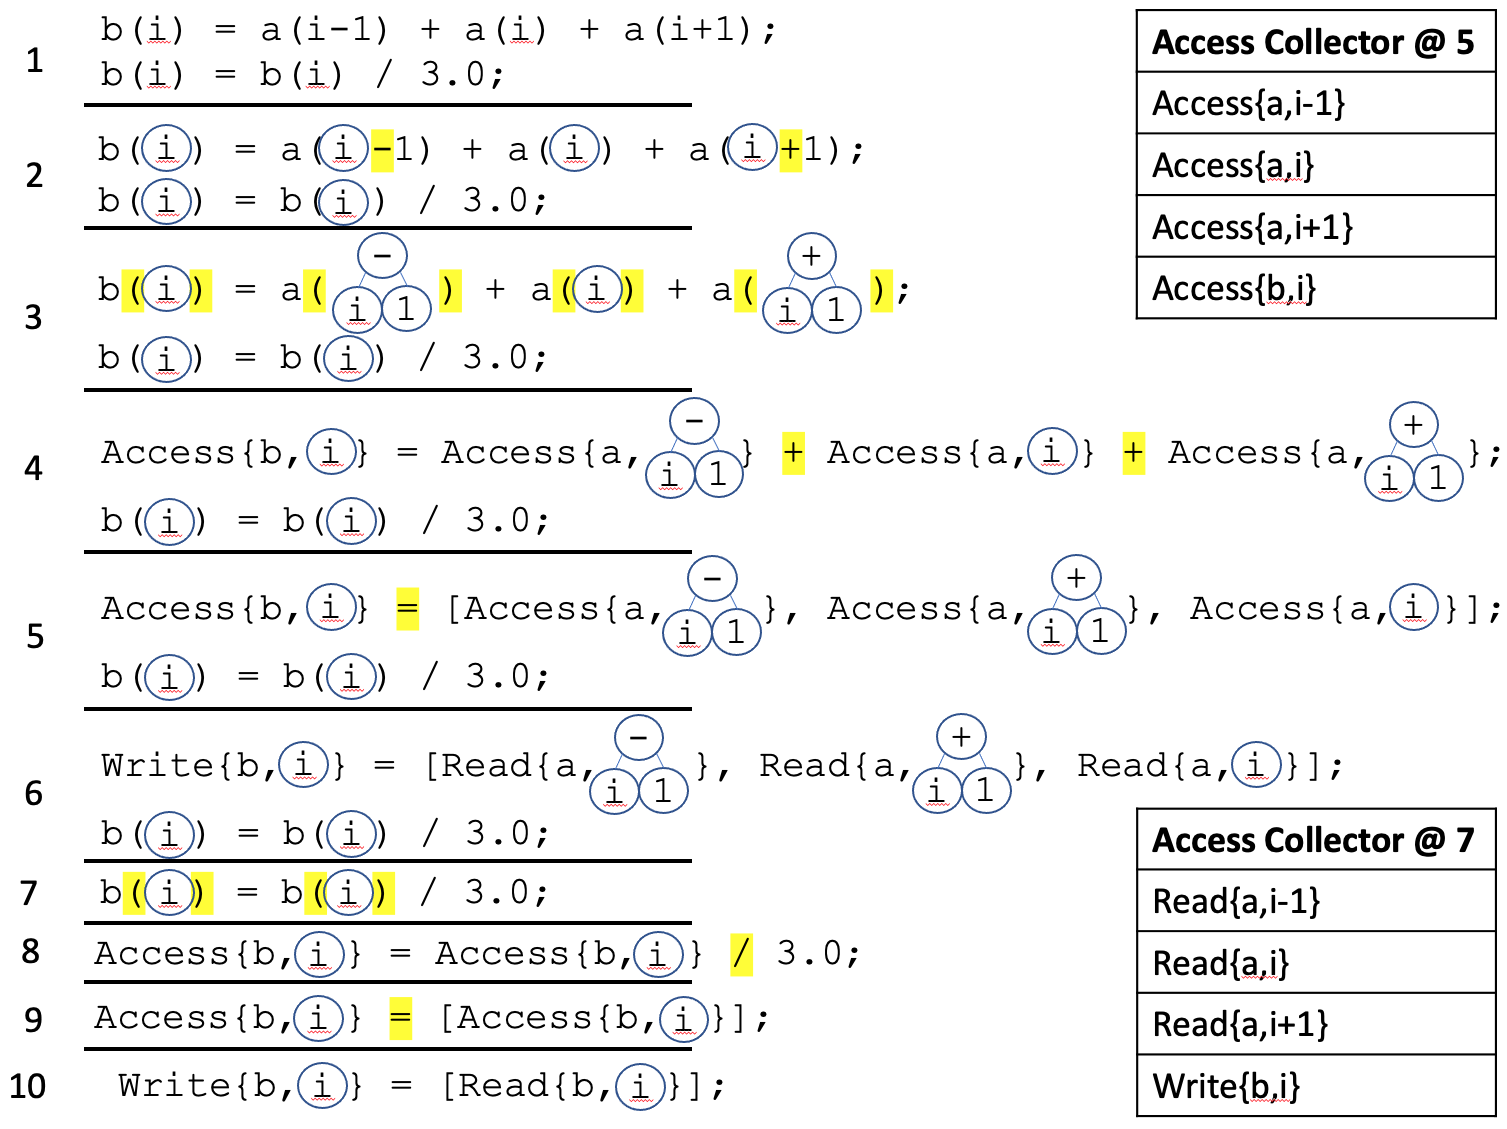
\includegraphics[width=\linewidth]{SymExecProcess.png}
\caption{Symbolic evaluation of a kernel lambda. 
Indexing expressions are evaluated first, then accesses, then statements in terms of accesses.
As assignments are evaluated, the accesses are marked as reads or writes.
Accesses are tracked using the access collector.}
\label{symExec}
\end{figure}

Figure~\ref{symExec} shows the process of symbolically evaluating the body of a lambda. 
We break kernel symbolic evaluation into two contexts: indexing and accessing. 
Indexing encompasses the representation and storage of index expressions, like
\verb.i+1. in \verb.a(i+1)..
The symbolic evaluation must retain the entire structure of the index expression 
because the loop's
data access pattern must reflect the difference between \verb.a(i+1). and
\verb.a(i-1)..
Indexing evaluation is shown in steps 2 and 3 of Figure~\ref{symExec}.
Accessing encompasses the statement-level data access semantics of the kernels.
Unlike with indexing, only whether accesses are reads or writes matters,
not the entire structure of the statements.
For example, we need to know that the statement \verb.c(i) = a(i) + b(i).
reads \verb.a(i). and \verb.b(i). and writes \verb.c(i)., but not that it
adds \verb.a(i). and \verb.b(i)..
Access evaluation is shown in steps 4, 5, and 6 of Figure~\ref{symExec}.
Listing~\ref{ExpressionGrammar} shows the grammar for supported indexing expressions and access statements. 
Behavior for kernels that do not use this grammar is undefined.

Normal RAJA kernel execution only affects the states of its Views. 
However, symbolic evaluation should not change View states. 
Instead, it should only preserve the access information.
We achieve this by adding a class-wide access collector to the symbolic iterator. 
When symbolic accesses are evaluated, they are added to the collector, and updated as reads or writes when assignments are evaluated.
This access collector and its contents at steps 5 and 7 are shown to the right in Figure~\ref{symExec}, and the change can be seen between steps 5 and 6.
 
\begin{figure}[t]
\begin{lstlisting}[label={ExpressionGrammar},caption={EBNF Grammar to Support Symbolic Evaluation}]
start : Access Assignment Expression
Expression : Expression Operator Operand | Operand
Operand : Access | Int | Double | Iterator
Operator : + | - | * | / | %
Assignment : = | Update
Update: += | -= | *= | /= | %=

Access : Id '(' IndexExpressions ')'
IndexExpressions : IndexExpression | IndexExpression ',' IndexExpressions
IndexExpression : IndexOperand Operator IndexExpression | IndexOperand
IndexOperand : Int | Double | Iterator
\end{lstlisting}
\end{figure}

\paragraph{Related Work:}

Some work has experimented with overlapped tiling and other inter-loop
scheduling by hand.
Olschanowsky et al.~\cite{CathieSC14} showed that scheduling across loops and
reducing the temporary storage requirements led to problem size scaling and
significantly better performance in a CFD application.
Wahib and Maruyama~\cite{Wahib14} showed the importance of fusing kernel
computations for GPU execution.

Numerous approaches to scheduling across an outer ``time loop" in a stencil
code have been investigated as early as 1998~\cite{Bassetti98,Wonnacott00}.  
The Cactus project~\cite{Ripeanu2001,Allen00cactus-gtoolkit} and 
Ding and He~\cite{Ding2001} demonstrated  overlapped tiling by expanding
ghost cells in stencil computations. 
Wonnacott and Strout~\cite{Wonnacott13} review many other approaches to
time tiling for PDE codes that do explicit stepping versus implicit stepping.

A number of DSLs have been developed for specifying and
optimizing stencil computations.
The Pochoir work~\cite{Tang2011} embedded cache oblivious performance
optimizations to improve temporal locality in C++ code.
STELLA~\cite{Gysi2015}  and YASK~\cite{YASK2016} can specify and 
tune 3D finite difference stencil computations.
Rawat et al.~\cite{Rawat18} present a DSL called StencilGen for specifying
stencil computations.
They present algorithms that perform overlapped tiling within stencil
computations and heuristics for fusing between the computations for GPUs.
Their work demonstrates some possible performance benefits of scheduling
across stencil computations when targeting GPUs and CPUs. In contrast,
we present ways to enable and to control these optimizations across loops
in the context of a more general, parallel library, specifically RAJA.

LIFT~\cite{Hagedorn2018} is a data parallel, functional intermediate
representation that supports dense computations and stencil computations.
Once a computation written in a DSL is transformed to LIFT, pattern-based
transformation can implement optimizations such as overlapped tiling and
target many different architectures.
Krishnamoorthy et al.~\cite{Krishnamoorthy07} present an automated tiling
technique for stencil computations in which neighboring tiles perform
overlapping computations, which reduces communication and improves load
balance.

%[Image processing pipelines, which are also stencil applications.  
Embedded DSLs for image processing pipelines, such as
Halide~\cite{Ragan-Kelley2012,Ragan-Kelley2013} and
PolyMage~\cite{Mullapudi2015}, support orthogonally specifying and
scheduling stencil computations.
By exposing separate mechanisms for scheduling them, PolyMage supports
various scheduling, fusion, and tile size selection
algorithms~\cite{Mullapudi2016,Jangda2018,Adams2019}.
%BRANDON: Adding differentiation
However, using these embedded DSLs limits the expressible computation and requires prohibitive porting costs for large applications.
%Jangda and Bondhugula~\cite{Jangda2018} have developed heuristics for selecting tile sizes and
%fusing across image processing pipelines.
%[Compiler techniques that schedule across loops.  Requires code to be quite simple to be analyzed and 
%there have been a number of different heuristics for deciding when to fuse.]

%[DNNs optimizing across loops]
Several DSLs that specify deep learning neural network
architectures, including Halide extended for reverse mode automatic
differentiation~\cite{Li2018}, Tensor Comprehensions~\cite{Vasilache2018},
TVM~\cite{TVM2018} and Latte~\cite{TruongLatte2016} optimize across loops.
These DSLs have specific approaches to scheduling such as the Halide scheduling
algorithm for DNN~\cite{Yang2020}.
AutoTVM in TVM~\cite{Chen2019} learns how to schedule.
Frameworks like Delite~\cite{Sujeeth2014} for developing DSLs support 
cross-computation scheduling.

Although the DSL approach can better target a particular application domain,
our work to schedule across loops within RAJA supports a broader class of
applications.
Further, we provide a different separation of concerns. RAJA handles
performance portability while our loop chain extension handles scheduling
across loops.
DSL approaches handle all of the scheduling and targeting of architectures,
which leads to not all architectures being covered in some cases.

The most related work to this submission is work that more generally gathers
a computational representation and other work that aims to specify and
optimize loop chains.
Lightweight modular staging~\cite{LMS2012} presented an approach for gathering 
a representation of computation to enable scheduling across that implementation
in Scala.

Bertolacci et al.~\cite{Bertolacci2016,Bertolacci2019} propose extensions to
OpenMP pragmas to express and schedule loop chains.
The approach requires annotations about data accesses in the pragmas.
That work enables the specification of loop fusion and wavefront tiling. 

Luporini et al.~\cite{Luporini2019} has a similar goal of enabling the source
code that uses a library  (in this case Devito~\cite{Luporini2018}) to
schedule across loop computations that share data.
The loops in their case have indirect array accesses.
Thus grouping computations to improve data locality requires a run-time
inspection phase~\cite{Strout14IPDPS}.
Luporini et al. use various Python library interfaces to specify computations
using per-loop modularization and then a lazy-computation step that gathers
the loop descriptions and generates inspector-executor code for performing 
sparse tiling.
%% BRONIS: The following does not seem necessary; is not discussed
%% \begin{verbatim}
%%    with loop_chain(name, tile_size, fusion_scheme, ...):
%%        <some PyOP2 parallel loops>
%% \end{verbatim}
The key differences between their work and ours is that we leverage the view 
capability of RAJA to avoid needing to annotate how data is being accessed
in each loop.  
Instead, our symbolic analysis collects that information.

%End copy from RAJALC paper

\paragraph{Evaluation:}

Two metrics will be used to evaluate this proposed research: performance improvement and code delta. 
For both metrics, I will look at three variants of each evaluated code.
The first variant will be the original RAJA implementation. 
The second variant will be the original RAJA implementation, modified to implement the transformation by hand.
The third variant will implement the transformation using my contribution.

I will look at the execution time for single-node executions, comparing the execution times among the three variants. My contribution is expected to provide slightly lower performance improvements than the hand-implemented variant, due to overhead of the system.

I will also compare the difference in the source lines of code changed to implement each variant.
\paragraph{Preliminary Results:}
Preliminary results show similar performance results with drastically fewer code changes.


\subsection{Proposed Research: Data Transformations in RAJA}
\label{Sec:Work2}
The layout of data in memory is a key consideration in high performance computing applications.
From reducing cache and page misses to relieving pressure on memory bandwidth and avoiding inter-process communication, using a good data layout improves performance at all levels of an application.
RAJA's Views incorporate data layout as part of their initialization, allowing a user to try out different layouts without major refactoring costs.
However, some applications benefit from changing the data layout mid-computation to facilitate better locality.
Implementing such a mid-computation layout change in RAJA can improve performance, but is laborious to implement and lacks portability.
Thus, I propose introducing a lightweight, declarative API for changing data layouts between computations.
Furthermore, I propose developing a performance model for layouts using the loop bounds and data access order as input and a runtime interface that dynamically estimates performance to select an appropriate layout. 
These systems combine so that the model and runtime \enquote{fill in} layout choices
that the user did not specify.

\paragraph{Context and Background:}

Figure~\ref{DataLayoutImportance} shows the importance of a good data layout. 
The BadLayout column shows the execution time for a matrix multiplication where the three arrays are laid out opposite of their access order. 
The GoodLayout column shows the execution time for the same matrix multiplication when the arrays are laid out to match their access order.
The LayoutChange column shows the execution time of code that changes the layout from the bad layout to the good one.
Finally, the SwitchAndRun column shows the combined execution time of changing the layout from bad to good and then running.
As the graph shows, performance improves  significantly (72\%) simply by changing the data layout, and the cost of performing the layout change is small (<1\% of execution time). 


\begin{figure}
	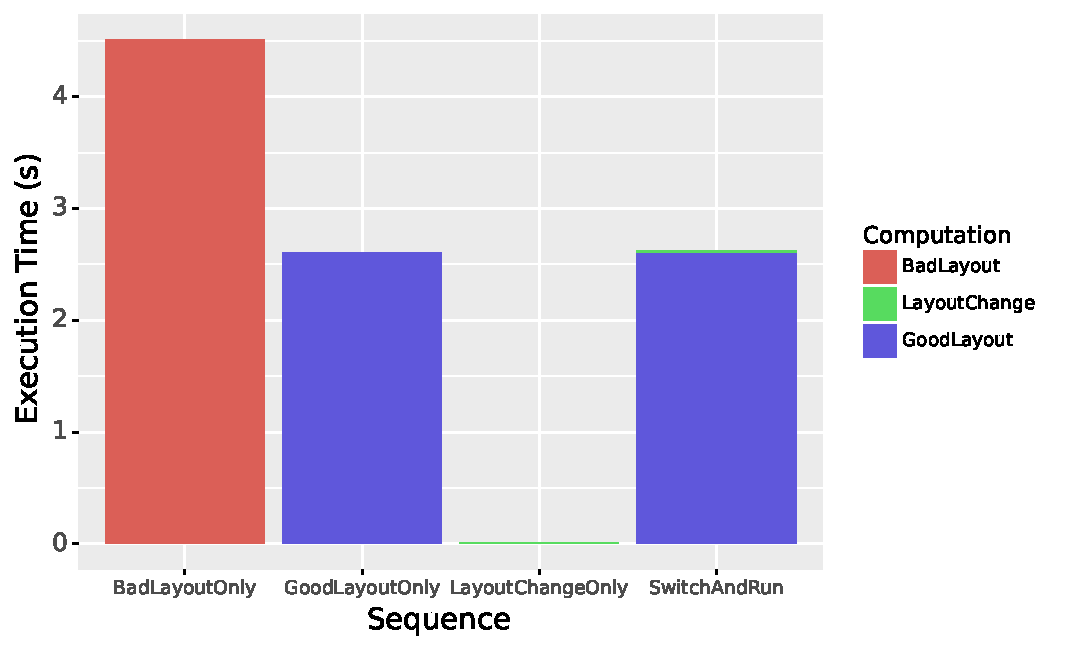
\includegraphics[width=\columnwidth]{IntroExampleGraph.pdf}
	\caption{Execution time for matrix multiplication using optimal and non-optimal data layouts and execution time for converting from non-optimal to optimal.}
	\label{DataLayoutImportance}
	%\Description[Matrix Multiplication Execution Time for Different Layouts]{A bar plot showing a "Bad Layout" column with execution time greater than the "Good Layout" and "Layout Conversion" columns combined.}
\end{figure}

\paragraph{Related Work}
Although controlling data layout is quite important, the options programmers have to control
data layouts in coordination with loop schedules have limitations.
Compiler optimizations such as loop permutation have been developed to change loop
schedules so that a loop traversal order better aligns with data layout.
However, general purpose compilers 
(1) have difficulties analyzing for the relationship between
data layout and schedule due to challenges like aliasing~\cite{hind2001pointer} and lack of multidimensional arrays in 
C/C++ languages; 
(2) do not generally expose fine-grained data layout or loop optimization
controls to users, leading to proposals to add pragma-based controls to OpenMP~\cite{kruse2019design} and Clang~\cite{kruse2018user}; and 
(3) typically do not optimize across multiple loops well.

The problem of inter-loop optimizations, especially those that balance parallelism and locality, has spawned many approaches. 
Approaches are often built into the compiler, lacking a user-accessible interface.
Some use loop schedule transformations alone~\cite{wolf1991data,mckinley1996improving}, while others consider data layout transformations as well~\cite{cierniak1995unifying,kennedy1995automatic,kandemir1998improving,  chen2005constraint, chen2005integrating, ozturk2011data}.
Other approaches develop or expand domain specific languages to expose controls to the user.
Many such approaches target stencil codes~\cite{henretty2011data,kronawitter2018automatic,luporini2018design} and image processing~\cite{ragan-kelley2013halide,mullapudi2015polymage}.

General purpose libraries like Kokkos and RAJA and programming languages like Chapel~\cite{diaconescu2007approach} give programmers some control over the data layout of multi-dimensional arrays. However, this support is limited to the point of initialization.
Thus, programmers must use that particular data format for the entire computation.
While a developer could change the data layout mid-computation in RAJA, the developer must either modify RAJA library code or use multiple arrays for the same data. 
Both options increase the code complexity and increase its fragility.
Even for the brave developer choosing one of these options, yet another obstacle remains: selecting the right combination of formats for the computation.
Even a modest computation of two loops using four 2D arrays has more than 200 combinations from which to choose, meaning trying out all possible options quickly becomes infeasible. 

\paragraph{Research Problems:}

\begin{itemize}
\item How do we formulate format selection for a loop chain in terms of constraints?
\item How do we enable users to specify format choices declaratively, and how do we represent those choices as constraints?
\item How do we define an objective function for such an ILP formulation?
\end{itemize}

\paragraph{Proposed Solution:}

\todo{rehash the ICS22 submission solutions}

\paragraph{Evalution:}

I will perform a similar evaluation to the loop schedule optimization proposal, looking at source lines of code added, removed, or modified; and changes in execution time among the different variants.

\paragraph{Preliminary Results}


\subsection{Proposed Research: Sparse Data Formats in RAJA}

Computations on sparse data are widespread. 
For example, any simulation using unstructured meshes require some sort of sparse representation.
While RAJA effectively separates concerns for dense codes, this is lost for sparse codes.
\todo{indicate why this is a probleM}
For instance, consider how data is indexed when using compressed sparse row (CSR). 
The data format is baked directly into the description of the computation, so changing the format of the data requires extensive refactoring of all parts of the kernel.
I propose extending RAJA's separation of concerns into the domain of sparse codes to enable the portable description of computations on sparse data.

\paragraph{Context and Background:}
\begin{figure}
\begin{lstlisting}[caption={CSR-stored sparse matrix vector multiplication},label={SpMVCSR}]
for(i = 0; i < N; i++) {
    y(i) = 0;
    for(j = A.rowptr(i); j < A.rowptr(i+1); j++) {
        y(j) = y(j) + A.val(j) * x(A.col(j));
    }
}
\end{lstlisting}
\end{figure}

A common kernel within sparse codes is the multiplication of a sparse matrix $A$ with a dense vector $x$.
Listing~\ref{SpMVCSR} shows how part of such a code is implemented when $A$ is stored using compressed sparse row.
These six lines elucidate how thoroughly intertwined the implementation is with the format of the sparse matrix $A$.
Note that even the accesses to $y$, ostensibly unconnected to $A$, are still based on values within $A$'s row pointer.
A developer seeking to change the storage format of $A$ must change almost the entire loop nest, a highly unscalable solution.

Existing approaches, such as the Tensor Algebra Compiler (Taco)~\cite{kjolstad2017tensor}, can portably represent SpMV and change the storage formats, but are restricted to computations with only reduction dependences.
This excludes common computations like direct solve.

No matter the system used to represent the computation, the importance of good layout choice is even greater for sparse computations.
While memory hierarchy means there are some benefits to be found in dense codes, dense arrays are constant time accessible ($O(1)$), so performance benefits come from a reduction of that nebulous constant $M$.
For CSR data, a poorly scheduled traversal can require a search for each access.
This means that proper format and schedule choice can reduce the algorithmic complexity of the computation.
\todo{reference to last subsection}


\paragraph{Research Problems:}
\begin{itemize}
    \item How do we extend the decoupling of data, operation, iteration space, and schedule description into the sparse context while maintaining idiomatically RAJA-like code? \todo{good to get feedback from bronis, dave, laura}
    \item How do we formulate format and schedule selection for sparse codes as an ILP problem?
    \item How do we estimate the cost of choosing different sparse formats and schedules?
    \item How do we support efficient iteration through sparse data without the ability to rewrite the operation for a particular format? 
\end{itemize}


\paragraph{Proposed Solution:}


\begin{figure}
\begin{lstlisting}[label={ForwardSolveC},caption={C-like implementation of forward substitution using Views}]
View2D A(N,N);
View1D x(N);
View1D b(N);

/* copy b into x */

for(int i = 0; i < N; i++) {
    for(int j = 0; j < i; j++) {
        x(i) = x(i) - A(i,j) * x(j);
    }
}
\end{lstlisting}
\end{figure}


\begin{figure}
\begin{lstlisting}[caption={Possible RAJA implementation of forward substitution.},label={ForwardSolveRAJA}]
auto lam = [&](auto i, auto j) {
    //note that references to A are format-independent
    x(i) = x(i) - A(i,j) * x(j);
};

using POL = KernelPolicy<
    statement::For<0,loop_exec,
        statement::For<1,loop_exec,
            statement::Lambda<0>
        >
    >
>;

auto seg0 = A.nonzeros(0);
auto seg1 = A.nonzeros(1) && RangeSegment(0,seg0.val());

auto segs = make_tuple(seg1, seg2);

auto knl = make_kernel<POL>(segs, lam);

auto chain = make_chain(knl);

//set the data format for A during knl
chain.set_data_format(knl,A,Format::CSR);

chain();

\end{lstlisting}
\end{figure}

The problem of decoupling has, ironically, a number of interrelated components.
First, what does it mean for code to be \enquote{idiomatically RAJA-like?}
I use a rather subjective notion: that a programmer familiar with RAJA recognizes the structure and semantics of the code. 
To achieve this, the description of a sparse computation should look as much like a dense code as possible. 

With this in mind, I turn to each component of the computation.
Starting with the previously mentioned coupling of the data format and operation, I recognize that through using Views, we already have a format-agnostic method for describing the computation. 
Thus, the lambdas should be written as if they were operating on dense Views, and all format specific indexing behavior should be abstracted into the View class itself. 
I suggest a similar approach for the schedule description as well.

The iteration space description requires more modification, illustrated by an example.
Listing~\ref{ForwardSolveC} shows a C-like implementation of the forward substitution step in a direct solve of the linear system $Ax=b$, a common kernel in sparse codes.
When $A$ is sparse, we do not need to iterate through all values in the dense iteration space.
Instead, we only need to iterate over the points where $A$ is nonzero. 
Thus, we need a way of reducing the iteration space to only the necessary points. 
I propose a symbolic iteration description API.
Views will have a method \verb.nonzeros(i). that represent the non-zero index values of the $i$th dimension. 
Segment dimensions will have a method \verb.value(). that represents the current value of that iterator, allowing for triangular and other shaped iteration spaces.
Finally, operator overloading will allow for the combination multiple ranges.
Line 15 of Listing~\ref{ForwardSolveRAJA} shows how this overloading could be used to combine the nonzero condition with the $j < i$ condition.

I now pivot to the problem of efficient iteration of the data.
Existing approaches to representing and optimizing sparse codes, such as Taco and the Sparse Polyhedral Farmework (SPF)~\cite{strout2016approach}, have an important feature that my proposed work does not: they are compilers.
While this adds complexity to the toolchain, it enables these approaches to perform rewriting steps based on the sparse format.
Thus, they can rewrite the access \verb.A(i,j). as some expression calculating a \verb.val_index. and then replacing the access to \verb.A. with \verb.val[val_index]..
In contrast, my proposed approach is incorporated into RAJA using only standard C++ features and compilers (GCC/Clang).
Because loop bodies in RAJA are specified as lambda closures, we cannot rewrite (or even directly inspect) the operations they perform.

To address this challenge, I lean on the wealth of information known about the computation, specifically the execution schedule provided by the user and the access information collected through symbolic evaluation. 
First, as part of the definition of a sparse format, one or more \enquote{efficient traversal orders} are declared. 
For example, CSR would have $(0,1)$ as a efficient traversal order, while CSC would have $(1,0)$.
Second, before the computation is executed, each sparse View in the computation will be prepared for the computation that is about to execute.
This preparation will change the backend behavior of the call operator.
If the computation is traversing the View's data in one of the specified efficient orders, the access function will guide the traversal through the data in an efficient manner.
Otherwise, the access function will perform the default behavior for the format, likely involving searching the index structure of the View.
Listing~\ref{BackendSketch} sketches some of these components for the CSR format. 


\todo{full example from code to model to choice}
\todo{how to describe sparse dependence / parallelism in sparse triangular solve within the policy}

\begin{figure}
\begin{lstlisting}[caption={Sketch of the backend for efficient iteration}, label={BackendSketch}]
View::prepare_for_traversal(Schedule schedule, SymAcess accessInfo) {
    auto traversalOrder = simplify(schedule, accessInfo);

    if(this->traversalFunctions.contains(traversalOrder)) {
        this->access_function = efficientTraversals[traversalOrder];
    } else {
        this->access_function = standard_access;
    }
}

CSR::standard_access(Index i0, Index i1) {
    auto col_lo = rowptr[i0];
    auto col_hi = rowptr[i0+1];
    auto val_index = search(col,col_lo, col_hi, i1);
    if(val_index != -1) {
        return val[val_index];
    }
}


CSR::efficient_traversal_access(Index i0, Index i1) {
    auto val_index = -1;
    if(last_i0 == i0) {
        val_index = last_val_index;
    } else {
        val_index = rowptr[i0];
    }

    while(col[val_index] != i1 && val_index < rowptr[i0+1]) {
        val_index += 1;
    }

    last_val_index = val_index;
    last_i0 = i0;
    last_i1 = i1;
    if(col[val_index] == i1) {
        return val[val_index];
    } else {
        return 0;
    }
}

CSR::efficientTraversals[[0,1]] = CSR::efficient_traversal_access;
\end{lstlisting}
\end{figure}

Another possible approach may be to attempt to simulate the rewriting of the lambda based on the symbolic evaluation results by translating the symbolic evaluation result into a format-specific access.
However, this is likely highly ineffecient, and may be obstructed by lambda type requirements.


\begin{figure}
\begin{lstlisting}[caption={Possible RAJA implementation of Sparse Matrix Multiply.}, label={SparseMMRaja}]
    
auto lam = [&](auto i, auto j, auto k) {
    C(i,j) += A(i,k) * B(k,j);
}
using POL = KernelPolicy<
    statement::For<0,loop_exec,
        statement::For<1,loop_exec,
            statement::For<2,loop_exec,
                statement::Lambda<0>
            >
        >
    >
>;

auto seg1 = A.nonzeros(0);
auto seg2 = B.nonzeros(1);
auto seg3 = A.nonzeros(1) * B.nonzeros(0);
auto segs = make_tuple(seg1,seg2,seg3);

auto knl = make_kernel<POL>(lam,segs);

auto chain = make_chain(knl);

chain.set_data_format(knl,A,Format::CSR);
chain.set_data_format(knl,B,Format::CSC);
chain.set_data_format(knl,C,Format::COO);

chain();

\end{lstlisting}
\end{figure}








\paragraph{Related Work}

\todo{libraries}
\todo{spf}
\todo{taco}
\todo{augustine2019}
\todo{taichi}


Magic table entries: support for arbitrary dependences, 

\subsection{Complete Example}

Start with the SpMM implementation from Listing~\ref{SparseMMRaja}.
This subsection will walk through my proposed approach step by step.
First, I will show how the model selects a data format. 
Then, I will show how the selected data format is applied to each View.

Before we start, I restrict the problem to N-dimensional compressed sparse fiber, with arbitray dimension ordering. 
In this restricted problem, compressed sparse row (CSR) is \verb.Format::CSF(0,1). and compressed sparse column (CSC) is  \verb.Format::CSF(1,0).

\paragraph{Format Model:}
This example's model has four values to identify:
\begin{itemize}
    \item Data format for A
    \item Data format for B
    \item Data format for C
    \item Execution nesting order
\end{itemize}
Generally, for each kernel in a chain, we model variables for each View's data format and the execution nesting order for that loop nest.


For the execution nesting order, the model will not be able to use different execution nesting orders, because the order is provided as a template argument. 
However, the system will be able to alert the programmer that there is a potentially better order choice.

Let's enumerate every variable in the model and what it's name indicates. 
\begin{itemize}
    \item \verb.A_fmt_0_1. True if A's format is ordering $(0,1)$, false otherwise
    \item \verb.A_fmt_1_0. True if A's format is ordering $(1,0)$, fales otherwise
    \item \verb.B_fmt_0_1. True if B's format is ordering $(0,1)$, false otherwise
    \item \verb.B_fmt_1_0. True if B's format is ordering $(1,0)$, fales otherwise
    \item \verb.C_fmt_0_1. True if C's format is ordering $(0,1)$, false otherwise
    \item \verb.C_fmt_1_0. True if C's format is ordering $(1,0)$, fales otherwise
    \item \verb.nest_0_1_2. True if the nesting order is $(0,1,2)$, false otherwise
    \item \verb.nest_0_2_1. True if the nesting order is $(0,2,1)$, false otherwise
    \item \verb.nest_1_0_2. True if the nesting order is $(1,0,2)$, false otherwise
    \item \verb.nest_1_2_0. True if the nesting order is $(1,2,0)$, false otherwise
    \item \verb.nest_2_0_1. True if the nesting order is $(2,0,1)$, false otherwise
    \item \verb.nest_2_1_0. True if the nesting order is $(2,1,0)$, false otherwise
\end{itemize}

Now let's consider the constraints on these variables. 
First, we have constraints so that there is only one format per View per computation. For A, this constraint looks like \verb.A_fmt_0_1 + A_fmt_1_0 = 1..
A similar approach generates constraints for nesting variables
\todo{format translation variables}

Finally, I need to describe the terms in the objective function.
I need to take into account the interaction between the variables in the model.
I assume there is only interaction between data format variables and nesting order variables. 
This means that for each combination of format variable and schedule variable, I run a dynamic microbenchmark accessing data with the format using the particular schedule. 
For the combo of \verb.A_fmt_0_1. and \verb.nest_0_1_2., let the execution time of the microbenchmark be \verb.ExecTime.
Further, let \verb.A_size. be the size of A. 
Then the term in the objective function will be \verb.(ExecTime * A_size) * A_fmt_0_1 * nest_0_1_2..

There will also need to be objective function terms for the cost of translating from one format to another. 

\paragraph{Applying the Format}
Once a format is selected, I need to propogate that format into the Views. 
This problem is tied with how the accesses are made efficiently. 

\section{Limitations}

\section{Project Schedule}
This section details the major milestones, deliverables, paper topics, and timeline for the completion of my dissertation. Note that the work from Sections \ref{Sec:Work1} and \ref{Sec:Work2} have already been submitted for publication.

\subsection{Tasks and Deliverables}

I break this project into a number of task-deliverable pairs.
While their presentation is strictly ordered, the true ordering is only partial. Progress on the tasks is co-iterative.

\paragraph{Evaluation Kernel Collection}
The first task is the curation of example computations for the evaluation of my approach. 
These kernels (which may be composed of multiple loop nests) will exhibit a variety of access patterns, dependence patterns, and scheduling choices. 
Along with the computations will be data representative of the applications from which the computations are derived. 
While some kernels may be derived from common linear algebraic operations, such as SpMV, these will be paired with data derived from applications that use the operation.
I aim to curate 100\% of the computations from codes related to fighting the climate crisis.

The deliverable associated  with this task is an open-source\footnote{See Section~\ref{Sec:DataPlan} for details} repository with the example computations implemented in RAJA in a format-\textit{dependent} way. 
The repository will provide a containerized instance that can be run using Docker.
This repository will constitute the baseline against which my system will be compared.

\paragraph{Sparse Data Formats}
The second task is the implementation of sparse data formats within RAJA.
To keep the scale of the project manageable in the time available, I restrict this step to a proof of concept for N-dimensional compressed sparse fiber (CSF) and Dense formats.  
While this implementation will not include performance modeling or automatic format conversion, it will form the basis upon which the modeling is built.
In addition to the implementation of the data formats themselves, this task also includes the implementation of the different access logic for efficient/inefficient traversal orders, as well as the preparation of Views for traversal.

The deliverable associated with this task is another open-source repository, this time containing implementations of the example computations in a format-\textit{independent} way.
It is likely that this deliverable will be the same repository as the previous task.
\paragraph{Model-Driven Format Conversion}
The third task is the implementation of model-driven format conversion within RAJA. 
As with the dense variant in Section~\ref{Sec:Work2}, this task will involve the normalization of each View's traversal order, development of the ILP constraints, dynamic cost estimation for using different formats, and development of the ILP objective function based on the cost estimations.

The deliverable associated with this task is a similar repository to the previous deliverables.
These implementations of the example computations will use the model-driven system to specify format changes.
Additionally, this deliverable will include an evaluation of the model accuracy, locating the model's choices in the space of all possible choices.

\paragraph{Written Dissertation}
The final task is the writing of the complete dissertation on the work I have undertaken during my PhD studies.
This task will also include writing and submitting a third paper to a peer-reviewed venue.
The deliverable for this task is a third peer-reviewed publication and my complete, defended dissertation. 
\subsection{Timeline}

\paragraph{Summer 2022:} 
I will be doing an internship at HPE working on the Chapel programming language~\cite{diaconescu2007approach} from May to August of 2022.
During this time, I will be focusing on two main tasks.
First, I will be working with climate scientists to explore how their codes may be ported from their current implementations into Chapel. 
While porting their code, I will be making special effort to extract example kernels from their codes that may be implemented in RAJA.
Second, I will be looking at how to incorporate the ideas from \ref{Sec:Work1} and \ref{Sec:Work2} into Chapel. 
Those approaches were designed to be applicable in a number of languages and this will be put to the test this summer.

During this time, I will also be working on implementing the sparse data formats within RAJA. While I aim to complete this task during the Summer, it may continue into the Fall.

Furthermore, in service of not entering Spring 2023 with no writing done, I will be participating in a daily writing activity.
Each work day, I will spend at minimum 15 minutes writing about the work I am doing.
From May through August, this amounts to 1,275 minutes of writing.
This will also assist in preparing me for a third submission to a peer-reviewed venue.
\paragraph{Fall 2022:} 
During the Fall of 2022, I will complete any remaining work on implementing the sparse data formats.
Additionally, I will implement the model-driven format conversion system.
I will continue the daily writing activity, with the expectation that the time spent writing will increase as the semester continues, as submissions for peer-reviewed venues are due in the last months of the fall and the first months of the new year. 

\paragraph{Spring 2023:}
The final semester of my studies will be spent focusing on evaluating my contributions, submitting a paper to ICS2023, and writing the final dissertation. 
The submission deadline for ICS is normally the end of January or the beginning of February, so the first month of the Spring 2023 semester will be focused on preparing that submission and the later months on writing my dissertation.

\section{Data Plan}
\label{Sec:DataPlan}
All code related to my dissertation will be open source under the Atmosphere Software License, which imposes enforcable divestment obligations on the relicensing of software~\cite{atmospherelicense}. 
\section{Conclusion}


\bibliographystyle{abbrv}
\bibliography{proposal}
\end{document}